\documentclass{article}

\usepackage{graphicx}

\title{Problem8 Report}
\author{Qi Liu}
\date{\today}

\begin{document}
	
\maketitle

\section{Morphological Operations}
Here we implement four kinds of morphological operations: erosion, dilation, opening and closing. Erosion defined as $A\ominus B=\{z|(B)_z\subseteq A\}$ and dilation defined as $A\oplus B=\{z|[(B)_z\cap A]\subseteq A\}$. Opening is just apply dilation after erosion which is $(A\ominus B)\oplus B$ and closing is the opposite $(A\oplus B)\ominus B$.

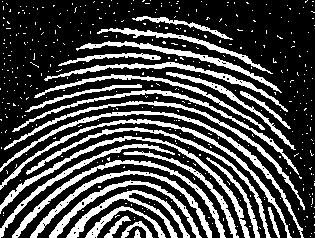
\includegraphics[width=0.33\textwidth]{../data/noisy_fingerprint.jpg}
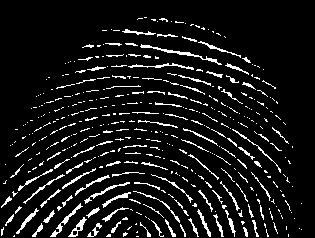
\includegraphics[width=0.33\textwidth]{../data/erosion_noisy_fingerprint.jpg}
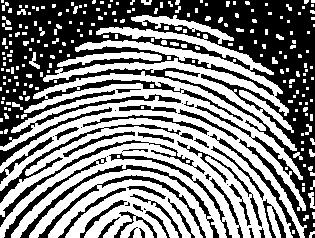
\includegraphics[width=0.33\textwidth]{../data/dilation_noisy_fingerprint.jpg}

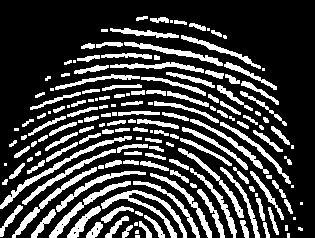
\includegraphics[width=0.33\textwidth]{../data/opening_noisy_fingerprint.jpg}
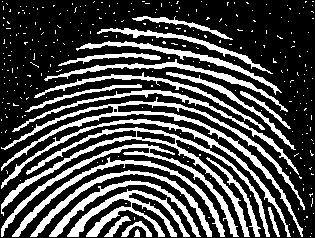
\includegraphics[width=0.33\textwidth]{../data/closing_noisy_fingerprint.jpg}

The first figure is the original one with white noise in the background and black noise in the fingerprint. The second is the result of erosion. The white noise has been removed but the black noise has been enhanced. The third one is the result of dilation, which removed the black noise but enhanced the white noise. The fourth and fifth are results of opening and closing which are better than just apply erosion or dilation. But the opening result has some gaps in the fingerprint and the closing result still has white noise in the background. 

\section{Boundary Extraction}
Boundary extraction is $A-(A\ominus B)$. The following figures show the result, we can see the performance is pretty good.


\includegraphics[width=0.5\textwidth]{../data/licoln_from_penny.jpg}
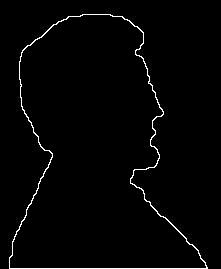
\includegraphics[width=0.5\textwidth]{../data/boundary_extraction_licoln_from_penny.jpg}

\section{Hole Filling}
Hole filling can be done by expanding from a pixel in the hole. The following figures are the result. We manually skipped the background to prevent a totally white image.


\includegraphics[width=0.5\textwidth]{../data/region_filling_reflections.jpg}

\includegraphics[width=0.5\textwidth]{../data/hole_filling_region_filling_reflections.jpg}

\section{Connected Component Extraction}
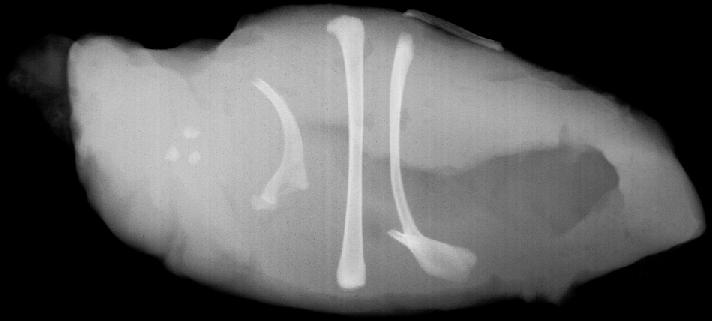
\includegraphics[width=0.5\textwidth]{../data/chickenfilet_with_bones.jpg}

\includegraphics[width=0.5\textwidth]{../data/connected_component_extraction_chickenfilet_with_bones.jpg}
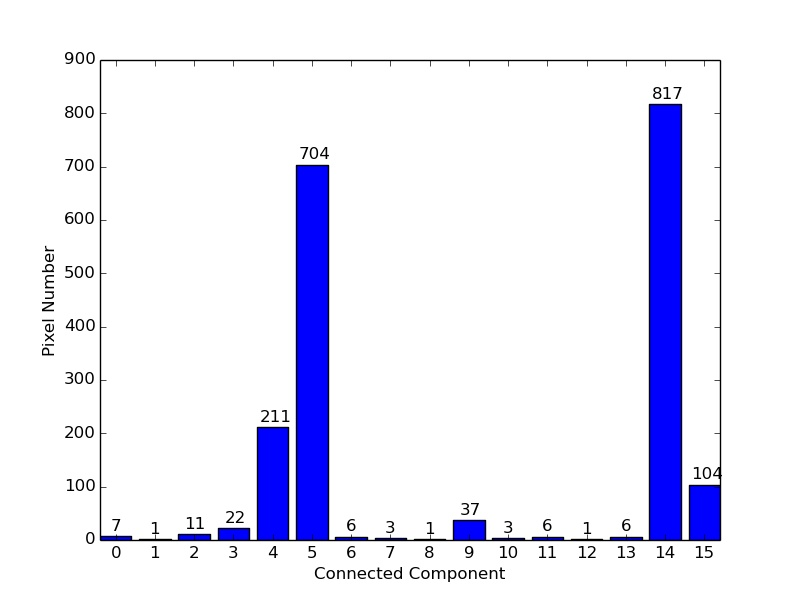
\includegraphics[width=\textwidth]{../data/connected_component_chickenfilet_with_bones.jpg}

The above figures show the result. The first one is the original image. We use a gray level threshold 210 to extract the bones and then apply erosion to get the second image. There are 16 connected components in the second figure, the details can be seen in the third one.

\end{document}